\section*{APPENDIX}
\subsection*{Short reminder on the NP-completeness theory}
A decision problem is a couple $(\Omega, S)$. $\Omega$ is described in
the section \textsc{Input} and is a set of words called instances of
the problem. $S$ is described in the section \textsc{Output} and is a
language included in $\Omega$. $S$ corresponds to the set of instances
for which the answer to the problem is ``yes'' (figure \ref{fig:problem}).

For example, the optimisation problem NST can be rephrased as the
following decision problem:\\
\textsc{Input:} A tree $T$, an integer $k \in \mathbb{N}$\\
\textsc{Output:} Yes if and only if there exists a self-nested tree $S$
such as the edit distancee between $T$ ans $S$ is less than $k$.\\
Here, each couple $(T,k)$ is an instance, and $\Omega$ is the set of all
the instances.
 
\begin{figure}[h]
  \centering
  \begin{subfigure}[b]{0.4\textwidth}
    \centering  
    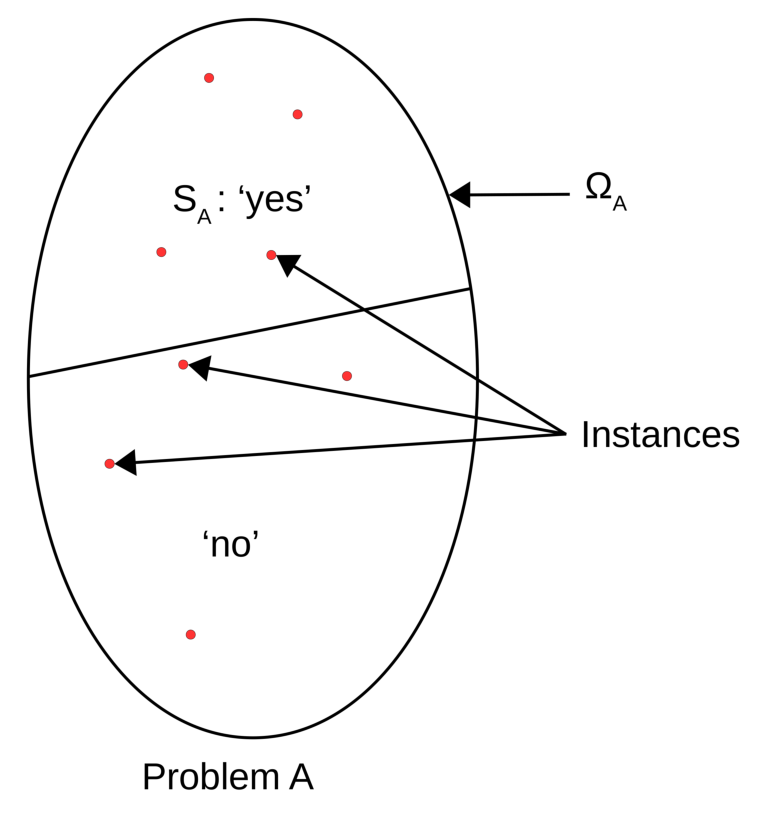
\includegraphics[width=.9\textwidth]{figures/problem.pdf}
    \caption{Algorithmic problem}
    \label{fig:problem}
  \end{subfigure}
  \begin{subfigure}[b]{0.5\textwidth}
    \centering
    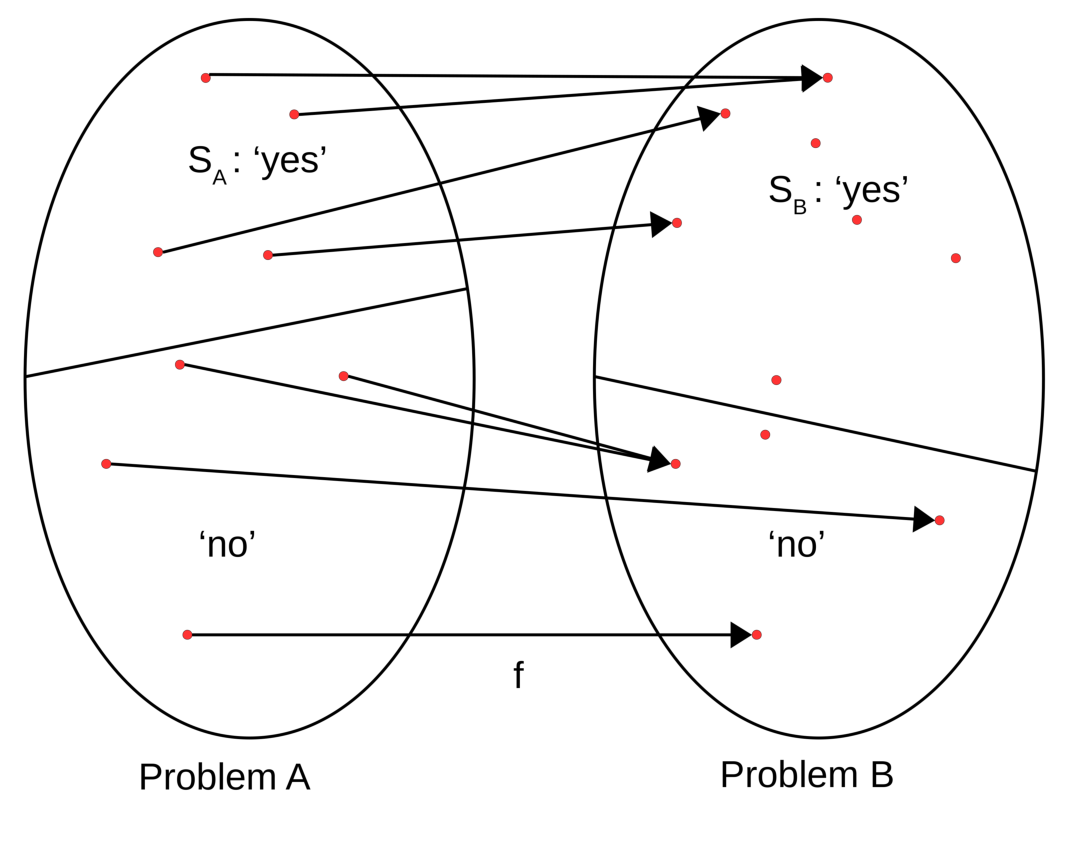
\includegraphics[width=\textwidth]{figures/reduction.pdf}
    \caption{Example of reduction}
    \label{fig:reduction}
  \end{subfigure}
%  \caption{Example of computation on the DAG}\label{fig:compute}
\end{figure}

The complexity class P is the class of problems for which there exists
a deterministic Turing machine deciding $S$ in a time polynomial to
the size of the instance. The complexity class NP consists of the
problems for which $S$ is accepted by a non-deterministic Turing
machine in polynomial time.

A reduction from a problem $A$ to a problem $B$ is a function
$f : \Omega_{A} \rightarrow \Omega_{B}$ such as for all instance
$\omega_{A}$ of $A$,
$\omega_{A} \in S_{A} \Leftrightarrow f(\omega_{a}) \in S_{B}$ (figure
\ref{fig:reduction}). As a result, if there exists a polynomial
reduction between $A$ and $B$ then $B$ is ``harder'' than $A$. Indeed,
if $S_{B}$ is accepted (respectively decided) by a Turing machine in
polynomial time, to accept (respectively decide) $S_{A}$ in polynomial
time, all there is to do is to apply the reduction to the instance of
$A$ and return the result computed by the Turing machine of the
problem $B$.
 
An algorithmic problem is called NP-hard if there exists a polynomial
reduction from each problem of the NP class to this one. The problems
that are both NP-hard and belong to the NP class are said to be
NP-complete.
